\documentclass{bioinfo}
\usepackage{amsmath}
\usepackage{amssymb}

\DeclareMathOperator*{\argmax}{arg\,max}
\newcommand{\s}{\mathbf{\Sigma}}

\newcommand{\nindiv}{601 }
\newcommand{\ngenes}{18,193 }
\newcommand{\nsnps}{1,125,747 }
\newcommand{\nsnpschr}{89,603 }


\copyrightyear{2016} \pubyear{2016}

\access{Advance Access Publication Date: Day Month Year}
\appnotes{Applications Note}

\begin{document}
\firstpage{1}

\subtitle{Genetics and population analysis}

\title[Fast SCCA]{Fast sparse canonical correlation analysis with flashpca}
\author[Sample \textit{et~al}.]{Gad Abraham\,$^{\text{\sfb 1,2}*}$
and Michael Inouye\,$^{\text{\sfb 1,2}}$}
\address{$^{\text{\sf 1}}$ Centre for Systems Genomics, School of
BioSciences, University of Melbourne, Parkville 3010, VIC, Australia and \\
$^{\text{\sf 2}}$ Department of Pathology, Faculty of Medicine, Dentistry, and
Health Sciences, University of Melbourne,\\ Parkville 3010, VIC, Australia.}

\corresp{$^\ast$To whom correspondence should be addressed.}

\history{Received on XXXXX; revised on XXXXX; accepted on XXXXX}

\editor{Associate Editor: XXXXXXX}

\abstract{\textbf{Summary:} Sparse canonical correlation analysis (SCCA) is a
useful approach for correlating one set of measurements, such as single
nucleotide polymorphisms (SNPs), with another set of measurements, such as gene
expression levels.  We present a fast implementation of SCCA, enabling rapid
analysis of hundreds of thousands of SNPs together with thousands of phenotypes.
Our approach is implemented both as an R package \texttt{flashpcaR} and within
the standalone command-line tool \texttt{flashpca}.\\
\textbf{Availability and implementation:}
\href{https://github.com/gabraham/flashpca}{https://github.com/gabraham/flashpca}
\\ \textbf{Contact:}
\href{gad.abraham@unimelb.edu.au}{gad.abraham@unimelb.edu.au}\\
\textbf{Supplementary information:} Supplementary data are available at
\textit{Bioinformatics} online.}

\maketitle

\section{Introduction}

Canonical correlation analysis (CCA) is a well-known statistical method for
multivariate analysis of two datasets~\citep{Hotelling1936}, such as genotype
data (single nucleotide polymorphisms) and multivariate phenotypes such as gene
expression levels. Approaches that consider one SNP at a time together with
multiple phenotypes have been shown to increase power to detect QTLs over the
simpler but often-used single-SNP/single-phenotype
approach~\citep{Ferreira2009}, particularly when analysing correlated phenotypes
that are modulated by the same genetic variation.

Analysis of multiple SNPs at a time is an attractive extension of approach,
however, standard CCA is not well-defined in this case, as typically the number
of samples is substantially lower than the number of SNPs ($n{\ll}p$).  One
solution is Sparse CCA (SCCA)~\citep{Witten2009b,Witten2009c,Parkhomenko2009},
an $L_1$-penalised variant of CCA where the number of variables that effectively
contribute to the canonical correlation can be tuned, making the problem
well-defined. Owing to the induced sparsity, SCCA can be useful for identifying
a small subset of SNPs and a small subset of the phenotypes exhibiting strong
correlations.  However, the rapidly increasing size and coverage of genotyping
arrays (exacerbated by genotype imputation), together with the availability of
large phenotypic datasets (transcriptomic, metabolomic, and others), makes it
challenging to perform analyses such as SCCA using existing tools.

We have developed an efficient implementation of SCCA that is capable of
analysing genome-wide SNP datasets (1M SNPs or more), together with thousands of
phenotypes (such as gene expression levels), as part of the tool
\texttt{flashpca}~\citep{Abraham2014}. The main code is implemented in
\textsf{C++} using the Eigen~3 numerical library~\citep{eigenweb}, and an
\textsf{R} implementation (package \texttt{flashpcaR}) is available via
RcppEigen~\citep{Bates2013}.

Here, we compare the SCCA implementation in \texttt{flashpcaR} and
\texttt{flashpca} with a widely-used implementation (\texttt{PMA},
by~\citet{Witten2013}), and demonstrate the substantial improvements in speed of
our tool, while achieving comparable or better cross-validated predictive power.

\begin{methods}
\section{Methods}

In standard CCA, we assume that we have two matrices $\mathbf{X}$ ($n \times p$)
and $\mathbf{Y}$ ($n \times m$), measured for the same $n$ samples.
We further assume that both $\mathbf{X}$ and $\mathbf{Y}$ have been
column-wise standardised (zero mean, unit variance).  For a single pair of 
canonical variables $a$ and $b$, CCA involves solving the problem
\vspace*{-10pt}
\begin{align}
\argmax_{a,b} & \frac{a^T \s_{XY} b}{
   \sqrt{a^T \s_{XX} a \; b^T \s_{YY} b}},
\label{eqn:cca}
\vspace*{-10pt}
\end{align}
where $\s_{XX}$ and $\s_{YY}$ are the covariance matrices of
$\mathbf{X}$ and $\mathbf{Y}$, respectively, and $\s_{XY}$ is the
covariance matrix of $\mathbf{X}$ and $\mathbf{Y}$. The solution is given by
the singular value decomposition of $\s_{XX}^{-1/2} \s_{XX}
\s_{XY}^{-1/2}$, with $a = \s_{XX}^{-1/2} u_1$ and $b =
\s_{YY}^{-1/2} v_1$, where $u_1$ and $v_1$ are the first left and right
singular vectors.

SCCA is typically run on high-dimensional data, where a useful assumption is that
the variables within $\mathbf{X}$ and $\mathbf{Y}$ are uncorrelated,
i.e., $\s_{XX}=\s_{YY}=\mathbf{I}$~\citep{Parkhomenko2009},
hence, $a = u$ and $b = v$. Thus, SCCA involves solving a simplified form of CCA,
\vspace*{-6pt}
\begin{align}
\argmax_{u,v} &  \quad u^T \s_{XY} v \notag \\
 & \mbox{s.t. } ||u||_2^2=1, ||v||_2^2 = 1, ||u||_1 \le s_u, ||v||_1 \le s_v,
\label{eqn:scca}\vspace*{-10pt}
\end{align}
where $u$ and $v$ are the left and right canonical vectors, 
and $s_u$ and $s_v$ are constraints on the $L_1$ norms
of canonical vectors.

The problem can be converted into the penalised (Lagrangian) form, making it
solvable using iterative soft-thresholding~\citep{Parkhomenko2009}, which we
employ here.  Unlike standard CCA, SCCA is well-defined even when $n{<}\min \{p,
m\}$, and induces sparse canonical vectors, depending on the choice of $L_1$
penalties: higher penalties lead to higher sparsity. The optimal set of
penalties can be found via cross-validation: the data (both $\mathbf{X}$ and
$\mathbf{Y}$) are split into training and test sets, SCCA is run on the training
set $(\mathbf{X}_{train}, \mathbf{Y}_{train})$ using a 2D grid of penalties, and
the pair of penalties that produce the highest correlations in the test set,
$\mbox{Cor}(\mathbf{X}_{test} u, \mathbf{Y}_{test} v)$, are selected.
Optionally, a new model may be fitted to the entire data using these penalties.

\enlargethispage{6pt}

\end{methods}

\begin{figure}[!tpb]
\centerline{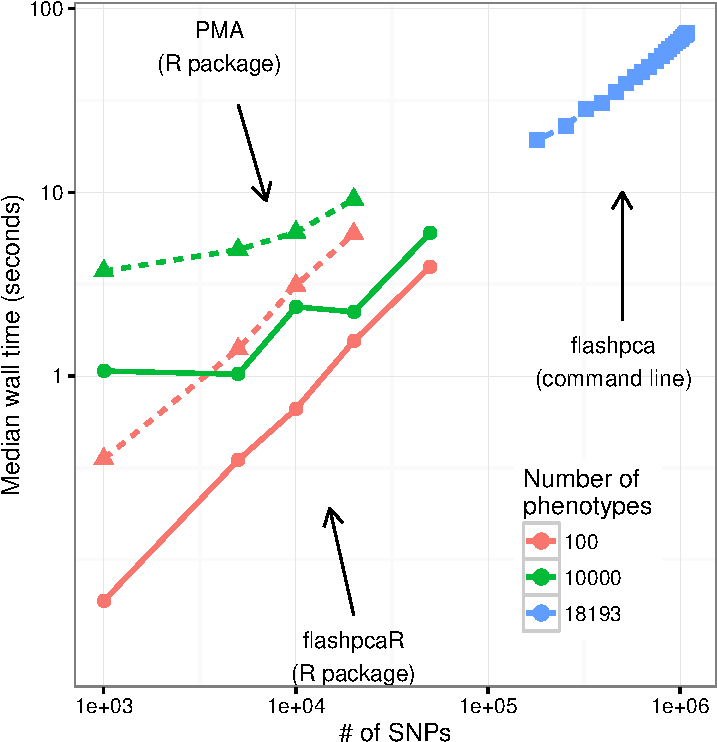
\includegraphics[width=0.49\textwidth]{scca_timing-crop.pdf}}
\caption{
Timing (median of 30 runs) of SCCA implemented in (i) the \texttt{flashpcaR}
(\textsf{R} package) and (ii) \texttt{flashpca} (stand-alone command-line tool),
compared with SCCA from \texttt{PMA}, using subsets of the HapMap3 dataset with gene
expression levels as phenotypes.
}
\label{fig:01}
\end{figure}

\section{Results}

To demonstrate our tool we utilised the HapMap3 phase III
genotypes~\citep{hapmap2010}, together with gene expression data of~602
individuals~\citep{Stranger2012}, with~1.4M SNPs and~47,000 gene expression
probes (out of which 21,800 probes were analysed by~\citet{Stranger2012} and
used in our analysis). After quality control (see Supplementary Material),
our data consisted of~\nindiv individuals, \nsnps SNPs, and~\ngenes gene
expression probes.

We first confirmed that \texttt{flashpcaR::scca} produced models competitive
with \texttt{PMA::CCA}, by comparing the best Pearson correlations produced
by each model in cross-validation.  Using chromosome~1 from the HapMap3
data (\nsnpschr SNPs), together with the~\ngenes gene expression levels,
we performed~5-fold cross-validation with a~2D grid of penalties (see the
Supplementary Material for details). The maximum of the average test-fold
Pearson correlations was identical for both \texttt{flashpcaR::scca} and
\texttt{PMA::CCA} ($\rho=0.044$).

Next, we compared the speed of three tools: (i) \texttt{PMA::CCA} (\textsf{R}
package), (ii) \texttt{flashpcaR::scca} (\textsf{R} package), and (iii)
\texttt{flashpca} (stand-alone command-line tool).
Figure~1\vphantom{\ref{fig:01}} shows a timing comparison between
\texttt{flashpcaR::scca} and \texttt{PMA::CCA} (using pre-computed SVD of
$\mathbf{X}^T \mathbf{Y}$ via \texttt{flashpcaR::flashpca}).
\texttt{flashpcaR::scca} was ${\sim}9\times$ faster than \texttt{PMA::CCA}, with
a medium-sized analysis (20,000 SNPs and~10,000 gene expression levels)
completing in~1s for the former but~9s for the latter.  For performing a
$20\times20$-penalty grid search in 10-fold cross-validation (assuming a single
core), this would translate to~${\sim}1$h for \texttt{flashpcaR}
versus~${\sim}9$h for \texttt{PMA}.

Whereas both \texttt{PMA::CCA} and \texttt{flashpcaR::flashpca} are
bound by the memory limitations of \textsf{R}, the command-line tool
\texttt{flashpca} allows much larger analyses. We ran analyses of increasing
size: chromosomes~1-2, 1-3, $\hdots$ , 1-22, up to all~\nsnps SNPs. The
stand-alone \texttt{flashpca} was able to complete an analysis of~\nindiv
individuals, ~\nsnps SNPs and~\ngenes gene expression levels in ${\sim}30$sec
(median of~30 runs), using ${\sim}9$GiB of RAM.

\vspace*{-12pt}
\section{Conclusion}

\texttt{flashpca} provides a fast implementation of sparse canonial correlation
analysis, making it possible to rapidly analyse high dimensional datasets.  For
datasets too large to fit in \textsf{R}, the command-line tool is available as
well, enabling fast analysis of~${>}1$M SNPs and thousands of phenotypes at a
time.  In addition to canonical correlation analysis of multiple quantitative
phenotypes, fast sparse partial least squares (sparse PLS) can be performed by
using a single phenotype at a time.

%\section*{Acknowledgements}

\vspace*{-12pt}
\section*{Funding}

This work has been supported by the NHMRC grant no.~1062227. GA was supported by
an NHMRC Early Career Fellowship (no.~1090462). MI was supported by a Career
Development Fellowship co-funded by the NHMRC and Heart Foundation
(no.~1061435).

\vspace*{-12pt}

\bibliographystyle{natbib}
\bibliography{paper}

%\bibliographystyle{achemnat}
%\bibliographystyle{plainnat}
%\bibliographystyle{abbrvnamed}
%\bibliographystyle{bioinformatics}
%
%\bibliographystyle{plain}
%

\end{document}

